\section{Experimental validation}
\label{sec:expe}

\subsection{Methodology}
\label{sec:exp-methodo}

This section briefly discusses our experimental setup for the evaluation of
\Moca.

All our experiment were run on  machines from Grid5000 \emph{Edel} cluster
\footnote{A full hardware description is available here
    \url{https://www.grid5000.fr/mediawiki/index.php/Grenoble:Hardware\#Edel}}.
    These machines are composed of $2$ quad core \texttt{Intel Xeon E5520} with
    $24 GB$ of RAM. Hyper threading was disabled during the experiment.

We deployed a \emph{Debian} \emph{Wheezy} environment running a Linux $3.X$
\DB{Linux version}.

We evaluate our tool on all the NAS Parallel Benchmarks~\cite{Jin1999} for
each benchmarks, we compare \Moca with the Pin~\cite{Luk05Pin} instrumentation
from Tabarnac~\cite{Beniamine15TABARNACRR}. This instrumentation traces every
memory accesses but record only the number of time each thread accesses to
each page, without any other information.

Each configuration of each plots was executed $30$ times. Each point shows the
\DB{wait for definitive expes}
arithmetic mean of all runs. The error bars in those plots represent the
standard error.

Except for the experiment on the influence of \Moca's parameters, on every
experiment, \Moca was run with it's default parameters. Which are a logging
process wakeup interval of $0.5s$ and a monitor thread wakeup interval
of $40ms$.
\DB{Check default params}

\DB{Results online ?}

\subsection{Experiments}
\label{sec:expe-ovh}

\begin{figure}[htb]
    \centering
    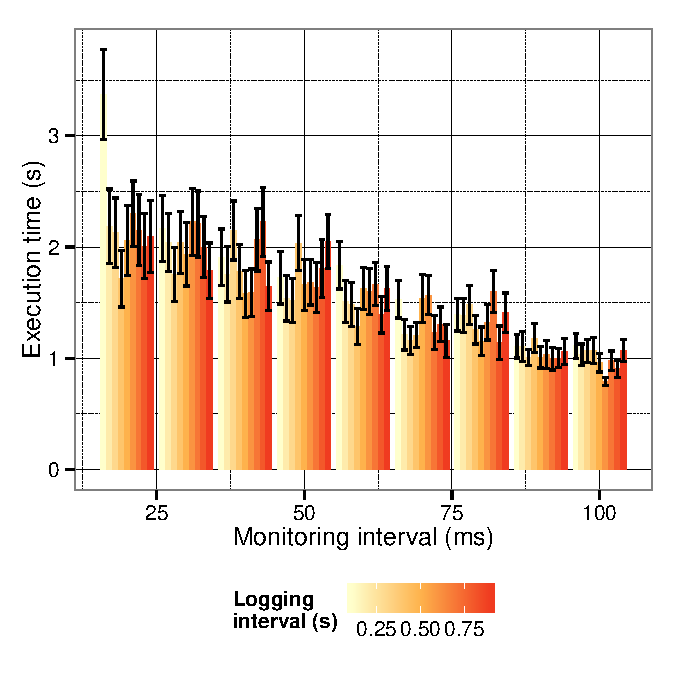
\includegraphics[width=\linewidth]{moca_param.pdf}
    \caption{Influence of the wakeup intervals on \Moca's overhead FT, class B.}
    \label{fig:param}
\end{figure}


\begin{figure}[htb]
    \centering
    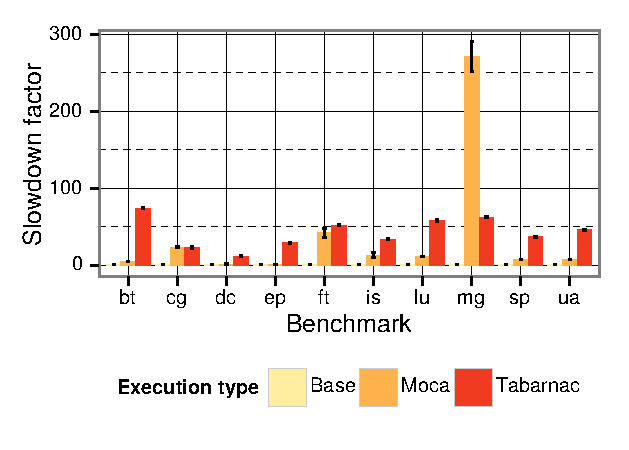
\includegraphics[width=\linewidth]{moca_overhead_nas.pdf}
    \caption{Slowdown of \Moca on the NAS parallel benchmarks compared to
    Tabarnac.}
    \label{fig:ovh}
\end{figure}

\begin{figure}[htb]
    \centering
    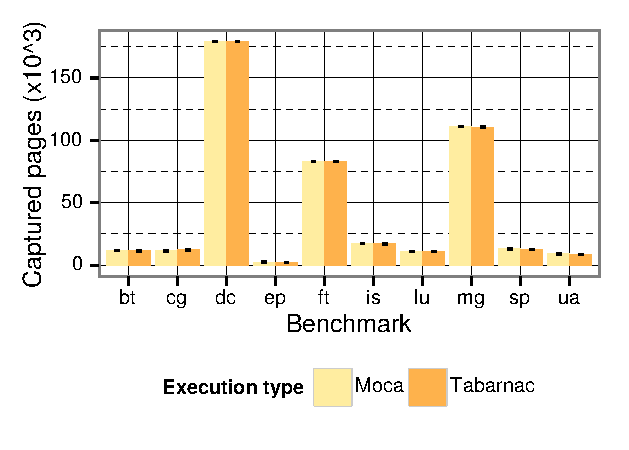
\includegraphics[width=\linewidth]{moca_pages_nas.pdf}
    \caption{Number of pages captured by \Moca and Tabarnac on the Nas
    Parrallel benchmarks.}
    \label{fig:pages}
\end{figure}

\begin{figure}[htb]
    \centering
    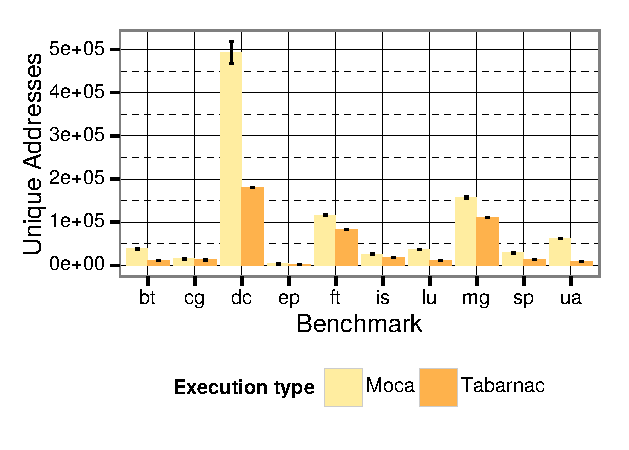
\includegraphics[width=\linewidth]{moca_addresses_nas.pdf}
    \caption{Number of unique addresses captured by \Moca and Tabarnac on the Nas
    Parrallel benchmarks.}
    \label{fig:addr}
\end{figure}

\begin{table}
    \centering
    \begin{tabular}{p{1.3cm}lcc}
        \toprule
        & & Granularity & Over set \\
        \cmidrule(lr){3-4}
        \multirow{4}{.8cm}{Trace precision}
        & Tabarnac & page & page \\
        & Mitos & ?? & none \\
        & MemProf & ?? & none \\
        & Moca & Byte & Page \\
        \midrule
        & & Time & Sharing and CPU localisation \\
        \cmidrule(lr){3-4}
        \multirow{4}{.8cm}{Complentary informations}
        & Tabarnac & no & thread sharing\\
        & Mitos & ?? & ?? \\
        & MemProf & ?? & ?? \\
        & Moca & yes & thread sharing + CPU \\
        \midrule
        & & Collection method & Architecture \\
        \cmidrule(lr){3-4}
        \multirow{4}{.8cm}{Portability}
        & Tabarnac & Instrumentation & Intel + AMD \\
        & Mitos & Hardware sampling & Intel + AMD + IBM \\
        & MemProf & Hardware sampling & AMD \\
        & Moca & Complete sampling & Any architecture\\
        \bottomrule
    \end{tabular}
    \caption{Comparison of different memory access collection
        tools: tabanarc\cite{Beniamine15TABARNACRR},
        Mitos~\cite{Gimenez14Dissecting},
        MemProf~\cite{Lachaize12MemProf} and MOCA}
        \label{tab:tools-comp}
\end{table}

\begin{itemize}
    \item Wakeup and logging interval => define defaults Figure~\ref{fig:param}
    \item NAS + Tabarnac => not worst than other tools Figure~\ref{fig:ovh}
    \item Number of Pages => No loss Figure~\ref{fig:pages}
    \item Number of uniq address => More precise Figure~\ref{fig:addr}
    \item Trace details see Table~\ref{tab:tools-comp}
\end{itemize}

    \subsection{Conclusion}
    \label{sec:expe-cncl}

    \begin{itemize}
        \item ``fast''
        \item ``precise''
    \end{itemize}
